\section{Throwing Booth}
\label{sec:hardware:throwing_booth}

The booth is constructed from Item aluminum profiles.
The background of the images shall remain the same, regardless of the current location.
Therefore, a white side wall opposite the camera is used.
When creating the booth design, care was taken to ensure that the size corresponds to the width of a table (\SI{750}{mm}).

The objects should be thrown as far away from the camera as possible to be able to take more pictures per throw.
To ensure that the objects are thrown through the field of view and as far away from the camera as possible, there is a hole in the rear wall as a target.
It is located on the right side of the rear wall, which is further away from the camera.
If the objects are shot through the hole in the rear wall, they end up in a net.

The rear panel is made of a \SI{5}{mm} thick ABS plate.
This material is robust and withstands the impacts of the throwing objects.
The side wall is made of foamed PVC.
Due to the manufacturing process, the plate is less smooth, which results in less light reflections and therefore better pictures.

The whole throwing booth is drawn in the CAD tool Inventor. It is designed with all its components using a 3D model.
The camera is mounted on an Item profile with an aluminum mounting adapter and protected from damage with an aluminum sheet.
Both components have slotted holes to allow fine adjustments during assembly.
Figure \ref{fig:booth} shows a 3D model of the throwing booth. 

\begin{figure}[h]
	\centering
	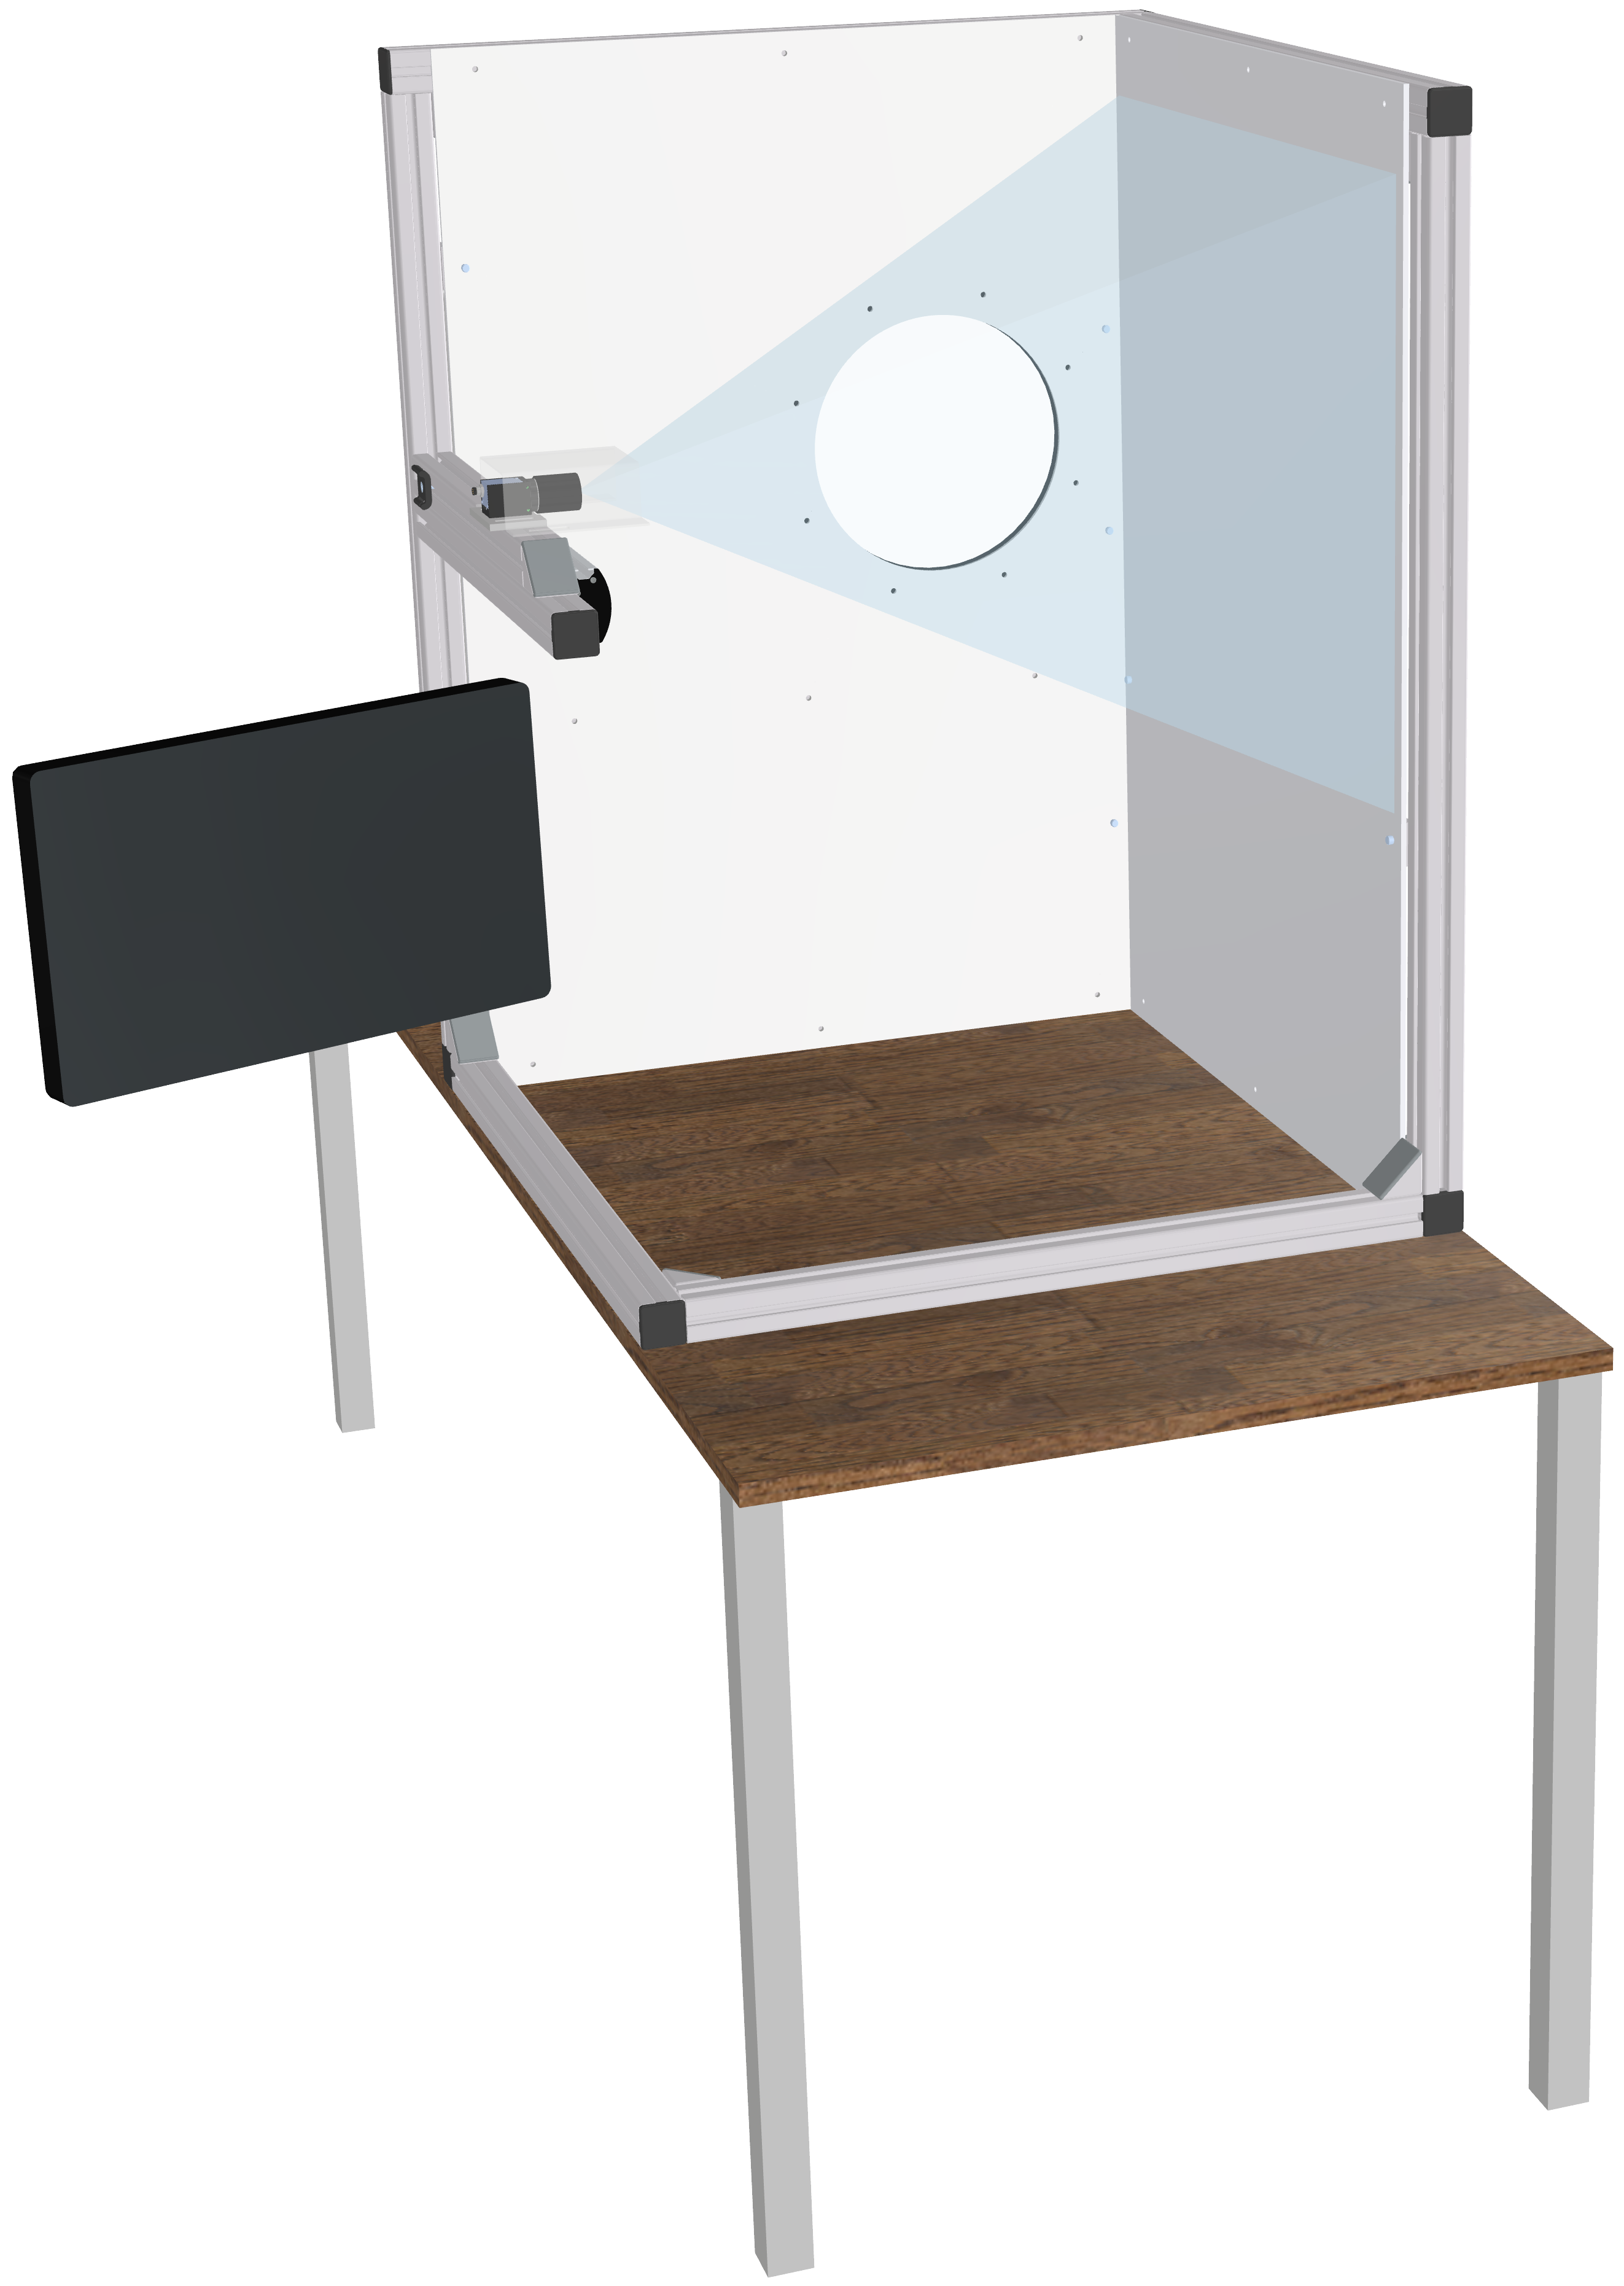
\includegraphics[width=0.5\textwidth]{graphics/top_assembly.png}
	\caption{3D model of the throwing booth}
	\label{fig:booth}
\end{figure}
